\section{Definition von SIEMs und Log-Analyse-Tools}

\gls{SIEM} ist das Ergebnis einer Kombination zwischen dem \glsfirst{SEM} und \glsfirst{SIM} \citep{Dorigo_SIEM}. Das Erste bezieht sich auf die Identifizierung, Bewertung, Beobachtung und den Bericht von Sicherheitsvorfällen mithilfe von verschiedenen Log Dateien \citep{techopedia_SEM}. Das Zweite ist eine Software, die bei der automatischen Sammlung von Loginformationen aus vielen Quellen, wie Firewall und Servern unterstützt \citep{techopedia_SIM}. Da die meisten \gls{SIEM}-Lösungen kostenpflichtig sind, existieren auch viele \gls{opensource} Log-Analyse-Tools, die eine ähnliche Aufgabe erledigen, ohne die Kernelementen von \gls{SIEM} zu besitzen. 

Log-Analyse-Tools sind meistens Anwendungen die Logdateien empfangen, speichern, bearbeiten und nach spezifisichen eingegebenen Regeln bewerten. Diese Tools unterstützen Programmierer und Systemadministratoren bei der Überwachung des Zustands eines Systems oder einer Software. Ein solches Tools kann Logdateien von verschiedenen \glsplural{Endpoint} und mit verschiedenen Formatierungen bekommen und editieren, so dass es schließlich einen Bericht oder eine Grafik erzeugt \citep{Korzeniowski_LATDef}. Die Nutzung dieser Tools schränkt sich nicht in dem Sicherheitsbereich ein, sondern kann für gesamte Rechenzentren nützlich sein.


In dem Universum des \gls{SOC} mischen sich verschiedene Begriffe, die manchmal zur Verwirrung führen, weil sie ähnliche Bedeutungen und Verantwortungen haben. \glsfirst{IDS}, \glsfirst{IPS}, \glsfirst{SIEM} und Log-Analyse-Tools werden von \textit{nonnative users}  und sogar von Spezialisten oft verwechselt, da ihre Aufgaben mehr Gemeinsamkeiten als Unterschiede haben. Um den Umfang dieser Arbeit wegen der zeitlichen Einschränkungen zu verringern, fassen wir kurz die Unterschiede zwischen denen zusammen und legen unsere Grenze auf den \glspl{SIEM} Lösungen und auf Log-Analyse-Tools fest. 

\newpage
\glsfirst{IDS} sind Software oder Hardware, die \glsplural{Cyberangriff} identifizieren und berichten. Sie haben eine passive Rolle, da sie die \glsplural{Cyberangriff} weder stoppen noch verhindern können. \glsfirst{IPS}allerdings haben sie eine aktive Haltung gegenüber \glsplural{Cyberangriff} - die sie automatisch behandeln können, indem sie Blocking-Mechanismen einschalten, um den Angriff zu stoppen \citep{Wendzel_IS}. Wie das \gls{IDS}, kann das \gls{IPS} auch Logdateien generieren, die von einer \gls{SIEM}-Lösung gesammelt werden können. \glsplural{SIEM} können einerseits die Logdateien von diesen und von anderen \glsplural{Endpoint} bekommen und diese nach vordefinierten Regeln bewerten, um dem \gls{SOC}-Team über Sicherheitsvorfälle zu informieren oder automatisch Maßnahmen ergreifen. Wie \glsplural{SIEM} bekommen Log-Analyse-Tools auch Logdateien, um Bericht oder Darstellung zu genieren. Ihre Nutzung ist aber nicht so spezifisch wie die von \glsplural{SIEM}. 

Die folgende Abbildung stellt didaktisch eine allgemeine Struktur von \gls{SIEM}-Lösungen dar:

\begin{figure}[H]
   \centering
   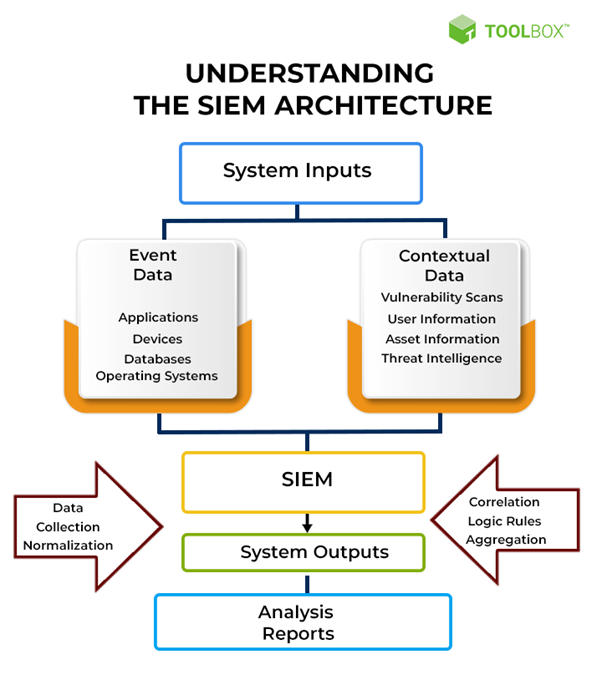
\includegraphics[width=0.55\textwidth]{assets/2_p1.png}
   \caption[Allgemeine Struktur von \gls{SIEM}]
   {Allgemeine Struktur eines \gls{SIEM}\\Quelle: \citep{Mohanan_What} }
   \label{fig:SIEM_Allg_Struktur}
   \centering
\end{figure}

\newpage
Aus dem Bild können wir feststellen, dass \glsplural{SIEM} für die Zentralisierung von Sicherheitsdaten zuständig ist. Diese werden dann bearbeitet und in einem oder mehreren Berichten dargestellt, damit das \gls{SOC}-Team schnellere und effektive Entscheidungen treffen können. Der Informationsfluss einer \gls{SIEM}-Lösung können wieder in der folgenden Abbildung dargestellt werden:

\begin{figure}[H]
   \centering
   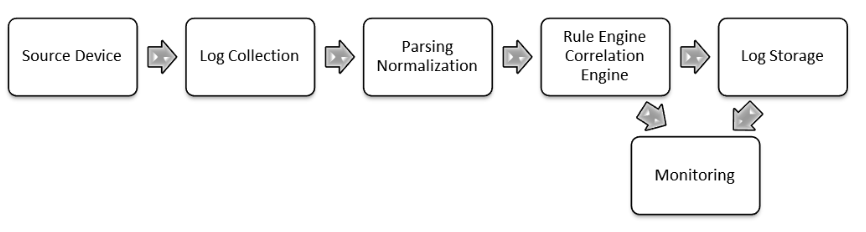
\includegraphics[width=0.8\textwidth]{assets/2_p2.png}
   \caption[Allgemeine Informationsfluss von \gls{SIEM}]
   {Allgemeine Informationsfluss eines \gls{SIEM} \\Quelle: \citep{Granadillo_SIEM} }
   \label{fig:SIEM_Allg_Informationsfluss}
   \centering
\end{figure}

Die folgende Abbildung zeigt eine allgemeine Architektur von Log-Analyse-Tools:

\begin{figure}[H]
   \centering
   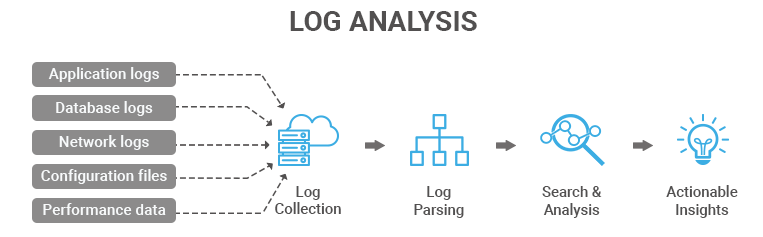
\includegraphics[width=0.8\textwidth]{assets/2.1_p2.png}
   \caption[Allgemeine Struktur von Log-Analyse-Tools]
   {Allgemeine Struktur von Log-Analyse-Tools\\Quelle: \citep{Tek-Tools_LGTArchitektur} }
   \centering
\end{figure}

Den Informationsfluss eines Log Analyse Tools bildet folgende Grafik ab:

\begin{figure}[H]
   \centering
   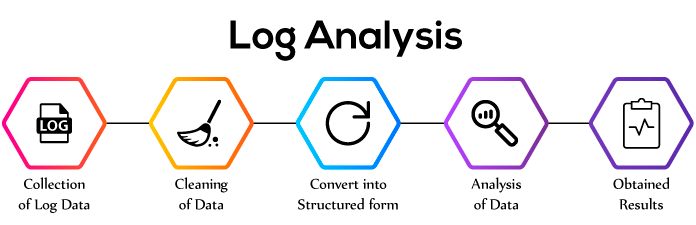
\includegraphics[width=0.55\textwidth]{assets/2.2_p2.png}
   \caption[Allgemeine Informationsfluss von Log-Analyse-Tools]
   {Allgemeine Informationsfluss von Log-Analyse-Tools\\Quelle: \citep{Neptune_LATInfoFluss} }
   \centering
\end{figure}

Aus bisheriger Beschreibung stellen wir fest, dass \gls{SIEM} viel mehr als eine Sammlung von Logdateien sind. Das Ziel dieser Software ist es die automatische Analyse zu ermöglichen, indem Daten kombiniert und bewertet werden können. In vielen Bereichen, wie Finanzen (\glsfirst{PCDISS}), Gesundheitswesen (\glsfirst{HIPAA}), sind \glsplural{SIEM}s eine gesetzliche Verpflichtung \citep{Jog_SIEM}. In Deutschland verpflichtet das zweite Gesetz zur Erhöhung der Sicherheit informationstechnischer Systeme Organisationen mit kritischen Infrastrukturen die Anwendungen solcher Lösungen, um Störungen der \glsfirst{CIA} zu verhindern \citep{BSI_ITSG}. Log-Analyse-Tools sind seinerseits allgemeine Tools zu der Speicherung, Anpassung, Bewertung und Darstellung von Logdateien, ohne dass sie sich auf die Sicherheitsebenen fokussieren.


\subsection{Existierende SIEMs Lösungen und Log-Analyse-Tools}
% über Splunk schreiben, state of the art, nicht open source, aber andere müssen ähnliche funktionaliten haben
Die existierenden \glsplural{SIEM} und Log-Analyse-Tools können in zwei Kategorien getrennt werden: \textit{\gls{Proprietary}} und  \textit{\gls{opensource}}. In folgenden Abschnitten präsentieren wir die proprietäre \gls{SIEM} Splunk, um einen Maßstab für unsere Auswahl zu definieren, wenn es um Funktionalitäten geht. Wir analysieren folgende \glsplural{SIEM} und Log-Analyse-Tools: 

\begin{itemize}[noitemsep]
   \item Prelude %(nein)
   \item AlienVault \glsfirst{OSSIM} %(nein)
   \item FortiSIEM %(nein)
   \item Elastic Stack %(nein)
   \item Grafana %(ja)
\end{itemize}

%\textbf{\textcolor{red}{Wie konnte ich Grafana hier erwähnen? Grafane ist eher allgemein und nicht so zu Alert orientiert, habe ich hier gefunden: \href{https://www.metricfire.com/blog/grafana-vs-splunk/}{Splunk x Grafana} und hier \href{https://www.researchgate.net/publication/350730340_Implementation_of_Grafana_as_open_source_visualization_and_query_processing_platform_for_data_scientists_and_researchers}{What is Grafana}}  }

\newpage
\subsubsection{Splunk}
Splunk von dem Unternehmen Splunk Technology wurde 2003 in den USA veröffentlicht \citep{Splunk_splunk}. Er gehört weltweit zu der meistverwendeten \gls{SIEM}-Software und gilt als \textit{State of the art} für andere ähnliche Lösungen \citep{Kazarov_Splunk}. Zu ihren Kunden gehören große Konzerne wie Airbus, Coca-Cola, Intel und die Deutsche Bahn. 

Splunk bietet laut seiner Webseite folgende Funktionalitäten an \citep{Splunk_SPE}:

\begin{itemize}[noitemsep]
   \item Skalierbare Datenplattform 
   \item Risk-based Warnmeldung  
   \item Bedrohungserkennung mithilfe von \glsfirst{ML} 
   \item Automatische Aktualisierung von der Bedrohungs- und Schwachstelle-Database 
   \item Unkomplizierte Installation und Anwendung 
\end{itemize}

Die allgemeine Architektur und der Informationsfluss von Splunk unterscheidet sich nicht von der oben dargestellten Struktur \ref{fig:SIEM_Allg_Struktur}, Seite \pageref{fig:SIEM_Allg_Struktur}, und Informationsfluss\ref{fig:SIEM_Allg_Informationsfluss}, Seite \pageref{fig:SIEM_Allg_Informationsfluss}. Da es sich hier um eine proprietäre Lösung handelt, lässt sich Splunk mit vielen anderen Funktionalitäten verwalten und erweitern. Die folgende Abbildung zeigt ein zusammenfassendes Diagramm über den Umfang des Informationsflusses von Splunk:

\begin{figure}[H]
   \centering
   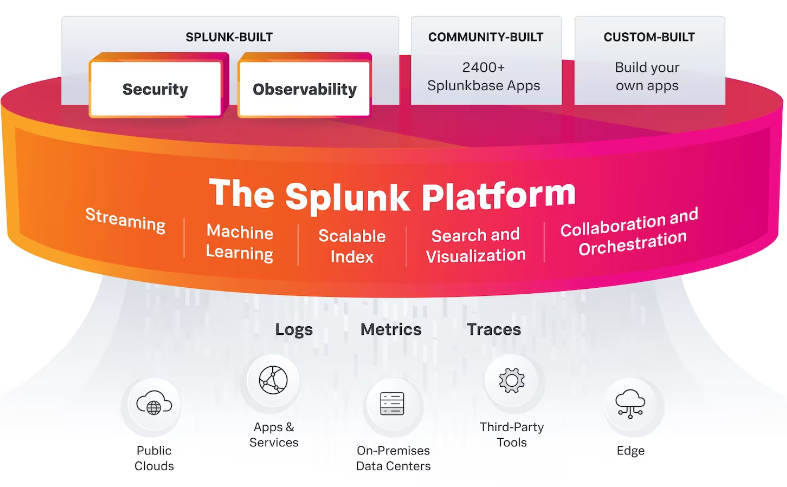
\includegraphics[width=0.7\textwidth]{assets/Splunk_informationsfluss.png}
   \caption[Allgemeine Informationsfluss von Splunk]
   {Allgemeine Informationsfluss von Splunk\\Quelle: \citep{Splunk_platform} }
   \centering
\end{figure}

In Splunk funktioniert die Bedrohungserkennung mithilfe von \glsplural{usecases}. Laut der Dokumentation existieren sie in folgenden Szenarien: Überwachung, Untersuchung und Erkennung. Die Software ist sowohl mit gls{mitre} Matrix als auch mit \glsfirst{CKC} für die Gestaltung ihrer \glsplural{usecases} integriert \citep{Splunk_usecases}. 

In einer spezifischen Arbeit wurden Angriffe auf einem System simuliert und schließlich mit Splunk analysiert, um Gefahren zu identifizieren und diese im Voraus zu sehen \citep{Su_SplunkDDOS}. In anderer Arbeit beschrieben die Autoren, wie eine Splunk-Instanz installiert und konfiguriert wurde, um spezifische \gls{bruteforce} zu erkennen \citep{Selvaganesh_SplunkBruteForce}.
 
\subsubsection{Prelude}
% suche nach Modulen, die man separat benutzen kann (Correlator)
Das im Jahr 2002 in Frankreich von Yoann Vandoorselaere freigegebene Tool Prelude zählt zu einer europäischen \gls{opensource} \gls{SIEM} Lösung. Laut dem Anbieter verfügt Prelude unter anderem folgende Funktionalitäten \citep{Prelude_SIEM}: 

\begin{itemize}[noitemsep]
   \item	Informationszentralisierung 
   \item	Datenaggregation und -Zusammenhang mit vordefinierten und von dem Nutzer angepassten Regeln 
   \item	Einbruchserkennungsmechanismen 
   \item	Datennormalisierung 
\end{itemize}

Die Anwendung besteht aus verschiedenen unabhängigen Modulen. Unter denen highlighten wir Warnmeldung, Archivierung, Analyse und Verwaltung. Das Erste gehört zu der zentralen Aufgabe dieser Lösung - es ist dafür zuständig, Daten zu empfangen, zu normalisieren, Zusammenhänge zu erschließen und Meldungen zu generieren. Das zweite Modul - Archivierung konzentriert sich auf die Speicherung und Verfügbarkeit der Daten. Zu dem Analyse-Modul gehören statistische Aufgaben und Darstellungen in verschiedenen Formaten. Das letzte Modul dient dazu, die Anwendung zu steuern, Nutzer zu erstellen dessen Rechte zu konfigurieren \citep{EC_Prelude}. 

Die folgende Abbildung zeigt die Integration verschiedener Module von Prelude und wie sie mit einander kommunizieren, um Analyse, Meldung und Speicherung zu generieren:

\begin{figure}[H]
   \centering
   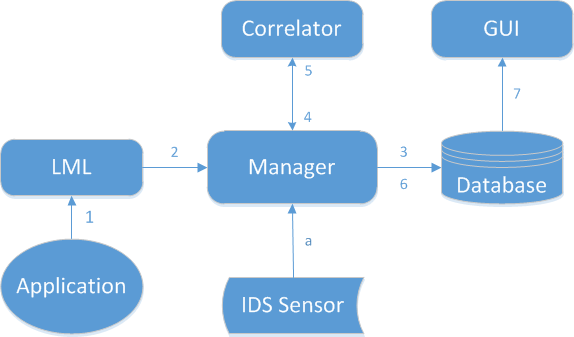
\includegraphics[width=0.5\textwidth]{assets/2_p3.png}
   \caption[Integration zwischen den Modulen von Prelude ]
   {Integration zwischen den Modulen von Prelude \\Quelle: \citep{Prelude_MU} }
   \centering
\end{figure}

Aus der Abbildung und der Dokumentation können wir folgenden Informationsfluss erkennen - die Daten werden von Endanwendung generiert und zum Loganalyzer (Prelude \glsfirst{LML}) geschickt, wo sie normalisiert und bewertet werden. Für solche Logs, wo es verdächtige Werte gibt, werden Warnmeldungen generiert. Diese Meldungen werden zum Manager Module weitergeleitet. Der Correlator oben sucht nach einem Zusammenhang zwischen anderen Daten. Das Ergebnis von Correlator wird wieder zum Manager geschickt und danach zu der Datenbank. Schließlich stehen die Berichte in dem User-Interface zur Verfügung \citep{Prelude_Doc}.

Die Architektur der Anwendung ermöglicht sowohl einen zentralisierten als auch einen dezentralisierten Aufbau. In der nächsten Abbildung sehen wir eine einfache Darstellung des Informationsflusses von Prelude:

\begin{figure}[H]
   \centering
   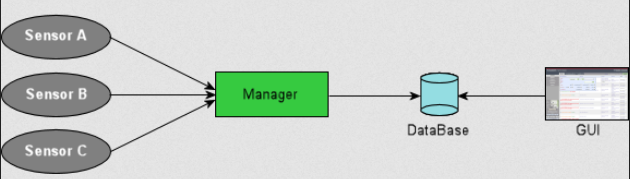
\includegraphics[width=0.7\textwidth]{assets/2_p4.png}
   \caption[Informationsfluss in Prelude]
   {Informationsflussin Prelude \\Quelle: \citep{Prelude_MU} }
   \centering
\end{figure}

In einer dezentralisierten Umgebung werden Daten von verschiedenen und getrennten Quellen generiert und bearbeitet. Schließlich können die Nutzer auf diesen Daten über eine \glsfirst{GUI} zugreifen.

\begin{figure}[H]
   \centering
   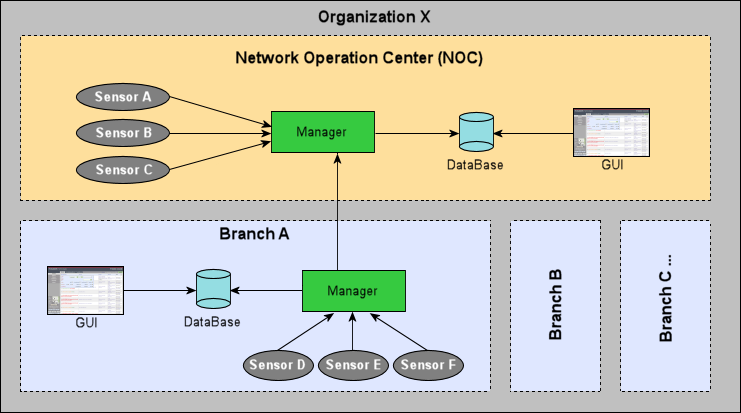
\includegraphics[width=0.8\textwidth]{assets/2_p5.png}
   \caption[Erweiterte Architektur von Prelude mit dezentralisierten Datenquellen und Datenverarbeitung]
   {Erweiterte Architektur von Prelude mit dezentralisierten Datenquellen Datenverarbeitung\\Quelle: \citep{Prelude_MU} }
   \centering
\end{figure}

Die wissenschaftliche Literatur über Prelude ist sehr eingeschränkt. Wenige Publikationen fokussieren sich auf die Entwicklung, Implementation und unternehmerische Anwendung dieses Tools. Eine Studie von 2021 versuchte dieses und zwei andere Tools (AlienVault und Cyberoam iView) anhand technischer und nutzerfreundlicher Kriterien zu vergleichen. Von diesn Kriterien highlighten wir folgende\citep{Grammatikis_Prelude}: 

\begin{itemize}[noitemsep]
   \item \textbf{technische Kriterien}
   \begin{itemize}[noitemsep]
      \item Echtzeige Leistung\textit{Real-time performance}, 
      \item Umfang und Flexibilität der Meldungen \textit{Range and flexibility of reporting}
      \item Zusammenhang von Warnmeldung \textit{Alert correlation}
   \end{itemize}

   \item \textbf{nutzerfreundliche Kriterien}
   \begin{itemize}[noitemsep]
      \item Vollständige Dokumentation \textit{Documentation comprehensiveness}
      \item Komplexität der Installation \textit{Complexity of the installation process}
      \item Komplexität der Einstellung \textit{Complexity of the system configuration}
   \end{itemize}
\end{itemize}

In den technischen Kriterien lag Prelude auf dem dritten Platz und in den benutzerfreundlichen Kriterien bekam Prelude den ersten. 

Auch in den nicht wissenschaftlichen Publikationen existiert eine begrenzte Anzahl von Texten über Preludes. Die existierenden Texte kommentieren ganz zusammenfassend die ausreichende Dokumentation und heben hervor, dass es eher eine in Europa verbreitete Lösung ist.

\subsubsection{AlienVault OSSIM}
AlienVault OSSIM ist eine im Jahr 2007 entwickelte \gls{opensource} \gls{SIEM} Lösung. Im Jahr 2018 wurden sie von der Firma AT\&T Communication gekauft  \citep{CBN_AV}. In der Beschreibung des Anbieters steht, dass er sie auch dabei unterstützt, Daten zu sammeln, zu normalisieren und zu bewerten. Er behauptet auch, dass sein Tool in der Lage ist, Schwachstellen und Angriffe zu erkennen, das Verhältnis zu beobachten und Datenzusammenhänge zu erschließen \citep{ATT_AVO}. 

AlienVault hat eine kostenpflichtige Version, die Alien Vault \glsfirst{USM} heißt. Auf der Webseite von AT\&T steht, dass es keine spezifische Dokumentation für die \gls{opensource} Version AlienVault OSSIM gibt, da viele Funktionalitäten von der anderen Version stammen \citep{ATT_AVO}. 

\newpage
Die folgende Abbildung zeigt das von dem Anbieter freigelegte Architekturdiagramm von der \gls{USM} Version:

\begin{figure}[H]
   \centering
   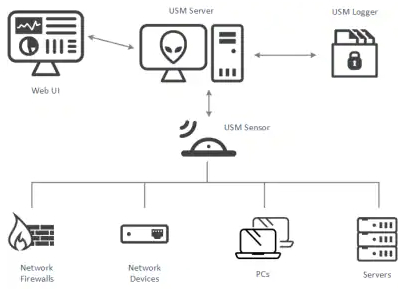
\includegraphics[width=0.6\textwidth]{assets/2_p6.png}
   \caption[Architekturdiagramm von AlienVault \gls{USM}]
   {Architekturdiagramm von AlienVault \gls{USM} \\Quelle: \citep{ATT_AVO} }
   \centering
\end{figure}

Laut der Website Comparitech steht AlienVault auf dem 13ten Platz von den bestbewertetsten \gls{SIEM}-Lösungen. Die Seite beschreibt auch, dass zu dem Tool einen \gls{IDS}, ein Verhaltensüberwachungssystem und einen Schwachstellen-Scanner integriert sind. Die Anwendung ist auch mit der Plattform \gls{OTX} verbunden - diese ermöglicht eine Teilung von Informationen über die Schwachstelle. Comparitech highlighted, dass die Anwendung wegen ihrer niedrigen Kosten besser für kleine oder mittelständige Unternehmen geeignet ist \citep{comparitech_SIEM}. 

Die Anwendung soll konsistenten Daten Zusammenhang anbieten und soll das Auftauchen von \gls{falsch positiv} vermeiden. AlienVault kommt auch mit vordefinierten Use-Cases, die dabei unterstützen, gewöhnliche Angriffsszenarien zu erkennen. Die Installation, die Einstellung und die Integration mit anderen Tools ist auch benutzerfreundlich \citep{Gomes_AV}. Aus einer anderen wissenschaftlichen Quelle fanden wir heraus, dass für viele Quellen eine manuelle Normalisierung der Logdatein notwendig ist \citep{Nabil_AV}. Die Anwendung hat aber einen zuverlässigen Berichtsmechanismus. 

Während unserer Recherche gab es wenig wissenschaftliche Literatur, die sich um AlienVault OSSIM kümmert. Die meisten Publikationen waren aus kommerziellen Quellen und diese konzentrierten sich auf eine kostenpflichtige \gls{SIEM}-Lösung von AT\&T..

\subsubsection{FortiSIEM}
FortiSIEM ist eine US-amerikanische \gls{SIEM}-Lösung von der Firma Fortinet. Fortinet kaufte im Jahr 2016 das Unternehmen AccelOps und dessen \gls{SIEM}-Lösung und benannte es zum FortSIEM \citep{Fortinet_Press}. 

Laut dem Anbieter hat FortiSIEM eine robuste Integration mit anderen Tools und lässt sich leicht und einwandfrei skalieren. Andere Versionen des Tools sind mit \glsfirst{ML} integriert, sodass die Anwendung auch Verhältnisanalysen durchführen kann \citep{Fortinet_Solutions}. Das Tool bietet auch eine umfangreiche und ausführliche Dokumentation an. Die nächste Abbildung zeigt die skalierbare Architektur des Tools:

\begin{figure}[H]
   \centering
   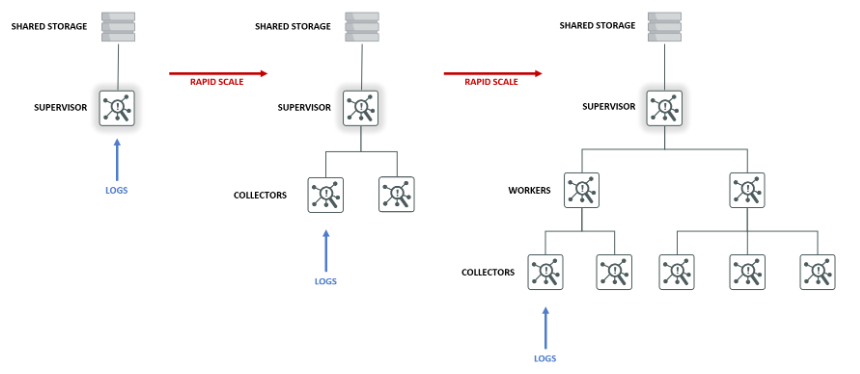
\includegraphics[width=1\textwidth]{assets/2_p7.png}
   \caption[Skalierbare Architektur von FortiSIEM]
   {Skalierbare Architektur von FortiSIEM \\Quelle: \citep{Fortinet_Arch} }
   \centering
\end{figure}

\newpage
Auch zu dieser \gls{SIEM}-Lösung ist die wissenschaftliche Produktion eingeschränkt. Eine von der gefundenen Publikation betont, dass FortiSIEM eine schnelle Erkennung von Angriffen anbietet und über  \glsfirst{NOC} Funktionalitäten verfügt \citep{Ramires_fortisiem}. Wie andere \glspl{SIEM} Lösungen, hat FortiSIEM folgende Funktionalitäten:

\begin{itemize}[noitemsep]
   \item Datensammlung und Normalisierung
   \item Daten Zusammenhang
   \item Generierung von Berichten
   \item Warnmeldungen
   \item Datenauswertung
\end{itemize}

\subsubsection{Elastic Stack}
Elastic Stack stammt aus der Verbindung von drei Tools: Elasticsearch, Logstash und Kibana. Das Erste ist eine Such-und Analyse-Maschine. Das Zweite ist eine serverseitige Anwendung zur Datenverarbeitung und -Weiterleitung. Schließlich Kibana \label{kibana} ist dafür zuständig, visuelle Darstellungen in einem Grafik-Format auszugeben (packt, 2019). Von diesen drei Tools Logstasch ist der einzige \gls{opensource} \citep{elastic_OSI}. Obwohl die anderen zwei 
kostenlos verwendet werden können, gehören sie nicht zu der \gls{opensource} Kategorie \citep{OpenSource_Def}. Dieses Tool besitzt viele Eigenschaften einer \gls{SIEM}-Lösung und wird von vielen SOC verwendet, ist aber für viele Experten, kein \gls{SIEM} für sich, da es über keine Warnmeldungssystem, Daten Zusammenhang und Vorfälleverwaltung verfügt \citep{Miller_ELK}. Diese und anderen Funktionalitäten lassen sich aber durch \glsplural{plugin} integrieren. 

\newpage
Das folgende Diagramm stellt die Architektur von Elastic Stack mit ihren integrierten Elementen dar:

\begin{figure}[H]
   \centering
   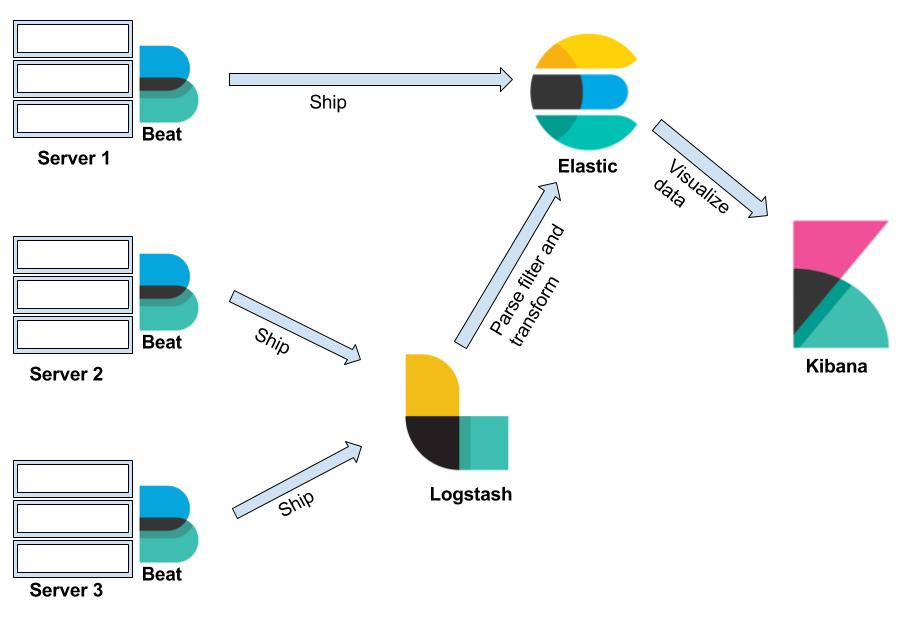
\includegraphics[width=0.8\textwidth]{assets/2_p8.png}
   \caption[Integration zwischen Elasticsearch, Logstash und Kibana]
   {Integration zwischen Elasticsearch, Logstash und Kibana\\Quelle: \citep{packt_elkstack} }
   \centering
\end{figure}

Die Beats auf dem Bild sind an der \glsplural{Endpoint} installiert und leiten Daten entweder zu Elasticsearch oder zu Logstash weiter, wo sie schließlich bearbeitet werden \citep{Jain_LMELK}. 

Ein Teil der wissenschaftlichen Literatur zeigt die Log Analyse-Funktionalitäten von Elastic Stack und die Unterstützung bei Normalisierung und Indexierung von Daten für eine lesbare Ausgabe \citep{Advani_elkstakc}. Die starke Skalierbarkeit wurde auch bei einer Studie erwähnt, wo Elastic Stack für Wi-Fi Logging eingesetzt wurde \citep{Wang_elkwifi}. 

Die offizielle Dokumentation von Elastic Stack betont, dass die Anwendung folgende Funktionalitäten besitzt \citep{elastic_docs}: 

\begin{itemize}[noitemsep]
   \item Datensuche, -Normalisierung, -Analyse und 
   \item Speicherung
   \item visuelle Ausgabe
\end{itemize}

Folgendes Diagramm aus der offiziellen Dokumentation zeigt die Aufteilung der Funktionalitäten pro Element von Elastic Stack:

\begin{figure}[H]
   \centering
   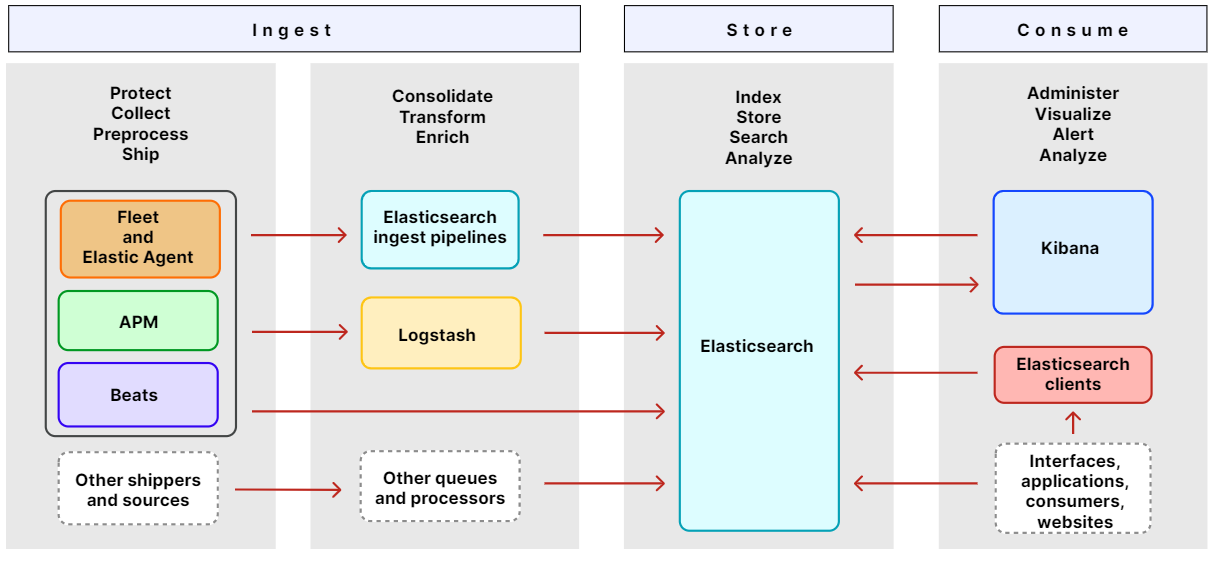
\includegraphics[width=0.8\textwidth]{assets/2_p9.png}
   \caption[Aufteilung der Funktionalitäten zwischen den Komponenten]
   {Aufteilung der Funktionalitäten zwischen den Komponenten\\Quelle: \citep{elastic_docs}}
   \centering
\end{figure}

Die wissenschaftliche Publikation über Elastic Stack ist vielfältiger als bei anderen recherchierten Tools. Es ist aber wichtig zu betonen, dass die Mehrheit von denen sich eher mit dem Logging als mit den \gls{SIEM}-Eigenschaften der Anwendung beschäftigt.

\subsubsection{Grafana}
Von allen recherchierten Lösungen ist Grafana die Einzige, die nicht als \gls{SIEM} dargestellt ist. Grafana wird aber als Plattform für Visualisierung von Daten beschrieben. Mit dem Tool ist es möglich eine Graphik zu erstellen und Meldungen zu definieren. Das Ziel der Anwendung ist, Information in einer einfachen und verständlichen Art und Weise zur Verfügung zu stellen \citep{redhat_grafana}.  

Im Jahr 2014 wurde Grafana von der Firma Grafana Labs veröffentlicht. Das Tool basiert auf Kibana3,\ref{kibana}. Ursprünglich sollte Grafana ein einfacheres Bearbeitungstool für Grafiken sein und ermöglichen, Datenanfragen unkomplizierter zu machen. Die neuste Version, 9.4.3. wurde im März 2023 veröffentlicht und bietet viele Funktionalitäten an. Es ist auch möglich das Tool mithilfe von  \glsplural{plugin} zu erweitern \citep{Oedegaard_historyGrafana}.. 

In der Webseite betont der Anbieter, dass Grafana die Zentralisierung und Zugang von Daten vereinfachen. Alle Art von Daten lassen sich analysieren und darstellen, von der Leistung von Anwendungen bis Verkaufsdaten und Krankheitsfällen. Die Anwendung soll auch den Zusammenhang von Daten ermöglichen, um wichtige Informationen herauszunehmen \citep{Grafana_Grafana}.

Grafana ist auch mit dem Logging Tool Loki und Promptail integriert. Promtail ist für Sammlungen der Logdateien und Weiterleitung an Loki zuständig. Promptail wird an jeden \gls{Endpoint} installiert. In Loki werden diese Logdateien ohne Index für den schnellen Zugriff gespeichert. Diese Daten können dann in Grafana mithilfe der \gls{abfragesprache} LogQL aufgerufen werden. Schließlich können Warnmeldungen mit spezfisichen Regeln generiert werden, die in Loki eingeführt werden \citep{Grafana_loki}. Auf dem Folgenden Bild wird die Struktur von Grafana Loki  dargestellt:

\begin{figure}[H]
   \centering
   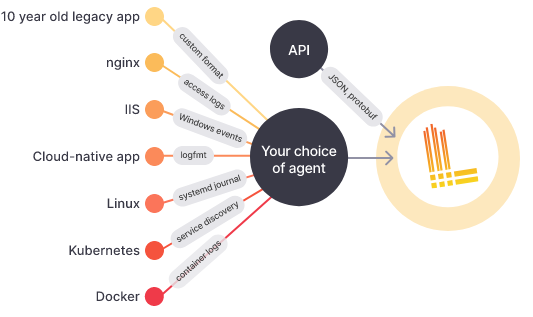
\includegraphics[width=0.8\textwidth]{assets/2_p10.png}
   \caption[Integration von Log-Quellen mit Promptail, Loki und Grafana]
   {Integration von Log-Quellen mit Promptail (links), Loki (mitte) und Grafana (rechts) \\Quelle: \citep{Grafana_Logs}}
   \centering
\end{figure}

Das Tool hat auch eine umfangreiche Dokumentation, die ausführlich erklärt, wie es zu installieren, bedienen und mit anderen Tools integrierbar ist. 

%\newpage
%Obwohl Grafana nicht spezifisch für den Sicherheitsbereich konzipiert wurde, kann das Tool so eingerichtet werden, dass spezifische Logdateien gesammelt, bearbeitet und analysiert werden. Die Warnmeldung lässt sich mit Regeln oder Filter definieren. In einer Recherche von 2022 wurde Grafana dafür benutzt, Daten aus Netzwerkverkehr graphisch darzustellen \citep{Manases_grafananetwork}. 

Die wissenschaftlichen Literatur über Grafana konzentriert sich eher auf die Anwendung des Tools für die grafische Darstellung von Daten als für ihre Nutzung in dem Sicherheitsbereich. Eine Recherche, z.B., wollte das Ergebnis von der Überwachung von Cloud-basierten Systemen, von Netzwerkaktivitäten und von Netzwerkverkehr mithilfe von Grafana darstellen \citep{Manases_grafananetwork}. In dieser Hinsicht gibt es wenige wissenschaftliche Arbeit, wo die Implementation und Integration von Grafana mit anderen Tools für den Sicherheitsbereich die Hauptfigur ist.

\subsection{Auswahlkriterien}
Eine umfangreiche \gls{SIEM} Software die viele automatische Lösungen für die Erkennung und Bekämpfung von Cyberangriffen würde perfekt für jede Situation passen. Da solche Lösungen meistens (oder alle) \gls{Proprietary} sind und nur für teure Preise angeboten werden, entschieden wir uns für die Anpassung eines \gls{opensource}Tools, das zu unserem Kontext und Einschränkungen gehört. 

Demnächst beschäftigen wir uns mit Grafana. Wir beschreiben, wie wir das Tool installieren, konfigurieren und mit verschiedenen Logdateien eingeben. Nachdem die Grundfunktionalitäten eingerichtet sind und einwandfrei funktionieren, generieren wir anhand der \gls{mitre} Matrix \glsplural{usecases} für die zukünftigen ausgewählten Angriffe. Unser Ziel ist Grafana so einzustellen, dass es in der Lage ist, die Muster dieser Angriffe zu erkennen und darüber zu berichten.
